% Required preamble packages for this section:
% \usepackage{booktabs}
% \usepackage{graphicx}
% \usepackage{siunitx}

\section{Benchmark Evaluation}

\subsection{Methodology}

The benchmark suite compares the priority-aware thread pool against the
Pacheco-style FIFO baseline pool using the repository's existing benchmark targets.
The fresh run used the locked configurations in the makefile: CPU-bound and
IO-bound workloads at 100,000 tasks with three trials, worker scaling at three
trials over 1, 2, 4, 8, 16, 32, and 64 workers, queue-operation throughput at
1,000,000 tasks with three trials, and the aging scheduler benchmark at five
trials. The machine reported 16 logical CPUs, AC power online, and the CPU
governor set to \texttt{performance} on all 16 CPUs. The recorded run revision
was \texttt{893a6b709dbe2f6d9f3ef44592268462f52cc34b}.

All summary tables report arithmetic mean plus sample standard deviation
($n-1$). The coefficient of variation is defined as
\[
  \mathrm{CV} = \frac{\mathrm{sample\ stddev}}{\mathrm{mean}} \times 100\%.
\]
For this evaluation, CV below 1\% is treated as highly stable, 1--3\% as
moderate variation, and above 3\% as noisy enough to require caution. Wall-time
throughput ratios are the source of truth. Perf counters are used only to
explain where time is spent.

\begin{table}[htbp]
\centering
\caption{Real-workload throughput comparison (mean $\pm$ sample stddev, $n=3$ trials)}
\label{tab:real_workload}
\begin{tabular}{lrrrr}
\toprule
Benchmark & Mine (t/s) & Baseline (t/s) & Ratio & CV (mine / base) \\
\midrule
CPU-bound (fib30, 100K) & 6\,096.4 $\pm$ 0.0 & 6\,141.6 $\pm$ 0.0 & 0.993x & 0.00\% / 0.00\% \\
IO-bound (64KB read, 100K) & 23\,733.2 $\pm$ 0.0 & 23\,400.5 $\pm$ 0.0 & 1.014x & 0.00\% / 0.00\% \\
\bottomrule
\end{tabular}
\end{table}

\begin{table}[htbp]
\centering
\caption{Worker scaling throughput (fib25 task, 10K tasks, $n=3$ trials)}
\label{tab:scaling}
\begin{tabular}{rrrr}
\toprule
Workers & Mine (t/s) & Baseline (t/s) & Ratio \\
\midrule
1 & 12\,684.1 $\pm$ 34.3 & 12\,179.6 $\pm$ 54.4 & 1.041x \\
2 & 25\,165.8 $\pm$ 36.1 & 24\,122.6 $\pm$ 27.8 & 1.043x \\
4 & 47\,761.9 $\pm$ 217.1 & 46\,211.5 $\pm$ 315.5 & 1.034x \\
8 & 87\,202.2 $\pm$ 2\,057.2 & 84\,599.2 $\pm$ 1\,733.6 & 1.031x \\
16 & 92\,100.7 $\pm$ 1\,750.7 & 89\,294.1 $\pm$ 287.3 & 1.031x \\
32 & 92\,022.8 $\pm$ 2\,975.9 & 89\,525.3 $\pm$ 606.3 & 1.028x \\
64 & 91\,952.1 $\pm$ 1\,454.9 & 89\,095.2 $\pm$ 519.0 & 1.032x \\
\bottomrule
\end{tabular}
\end{table}

\begin{table}[htbp]
\centering
\caption{Concurrent queue operations throughput (10K tasks per trial, $n=3$ trials)}
\label{tab:queue_ops}
\begin{tabular}{rrrr}
\toprule
Workers & Mine (ops/s) & Baseline (ops/s) & Ratio \\
\midrule
1 & 5\,920\,081.2 $\pm$ 76\,410.6 & 8\,469\,928.1 $\pm$ 190\,271.0 & 0.699x \\
2 & 5\,182\,658.2 $\pm$ 42\,833.2 & 7\,000\,034.1 $\pm$ 71\,943.0 & 0.740x \\
4 & 3\,733\,903.4 $\pm$ 14\,005.3 & 4\,992\,465.7 $\pm$ 41\,381.1 & 0.748x \\
8 & 1\,585\,654.7 $\pm$ 51\,711.0 & 2\,358\,960.3 $\pm$ 326\,279.8 & 0.672x \\
16 & 813\,579.9 $\pm$ 21\,630.2 & 845\,507.9 $\pm$ 2\,003.4 & 0.962x \\
\bottomrule
\end{tabular}
\end{table}

\begin{table}[htbp]
\centering
\caption{Coefficient of variation comparison (lower is more predictable)}
\label{tab:variance}
\begin{tabular}{lrrr}
\toprule
Benchmark & Mine CV (\%) & Base CV (\%) & Stability advantage \\
\midrule
CPU-bound & 0.00\% & 0.00\% & 0.00x \\
IO-bound & 0.00\% & 0.00\% & 0.00x \\
Scaling 1w & 0.27\% & 0.45\% & 1.65x \\
Scaling 2w & 0.14\% & 0.12\% & 0.80x \\
Scaling 4w & 0.45\% & 0.68\% & 1.50x \\
Scaling 8w & 2.36\% & 2.05\% & 0.87x \\
Scaling 16w & 1.90\% & 0.32\% & 0.17x \\
Scaling 32w & 3.23\% & 0.68\% & 0.21x \\
Scaling 64w & 1.58\% & 0.58\% & 0.37x \\
Queue 1w & 1.29\% & 2.25\% & 1.74x \\
Queue 2w & 0.83\% & 1.03\% & 1.24x \\
Queue 4w & 0.38\% & 0.83\% & 2.21x \\
Queue 8w & 3.26\% & 13.83\% & 4.24x \\
Queue 16w & 2.66\% & 0.24\% & 0.09x \\
\bottomrule
\end{tabular}
\end{table}

\subsection{Figures}

\begin{figure}[htbp]
\centering
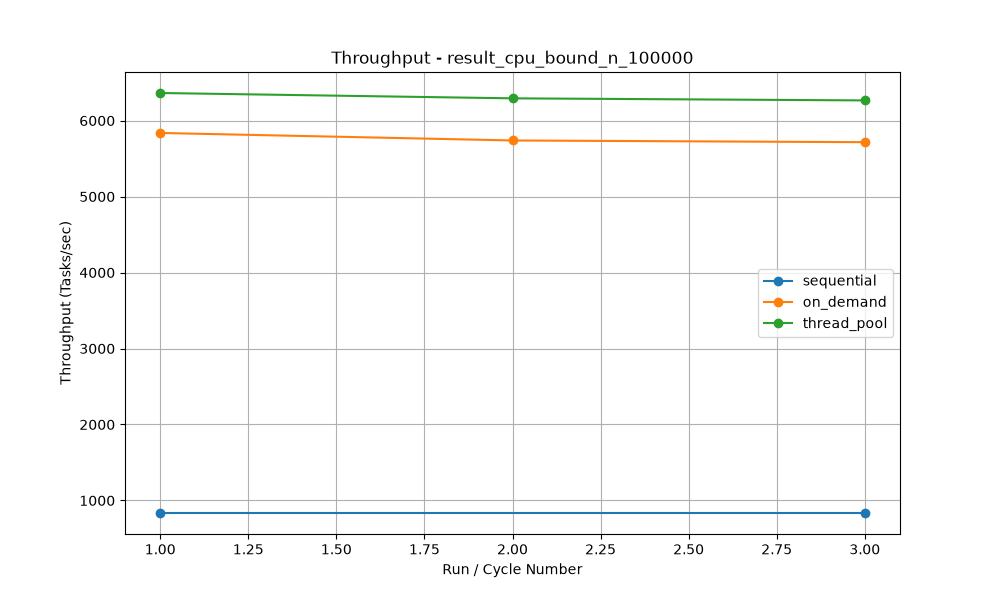
\includegraphics[width=0.82\linewidth]{benchmark/plot/cpu/throughput_result_cpu_bound_n_100000.png}
\caption{CPU-bound throughput for the priority thread pool.}
\label{fig:cpu_throughput}
\end{figure}

\begin{figure}[htbp]
\centering
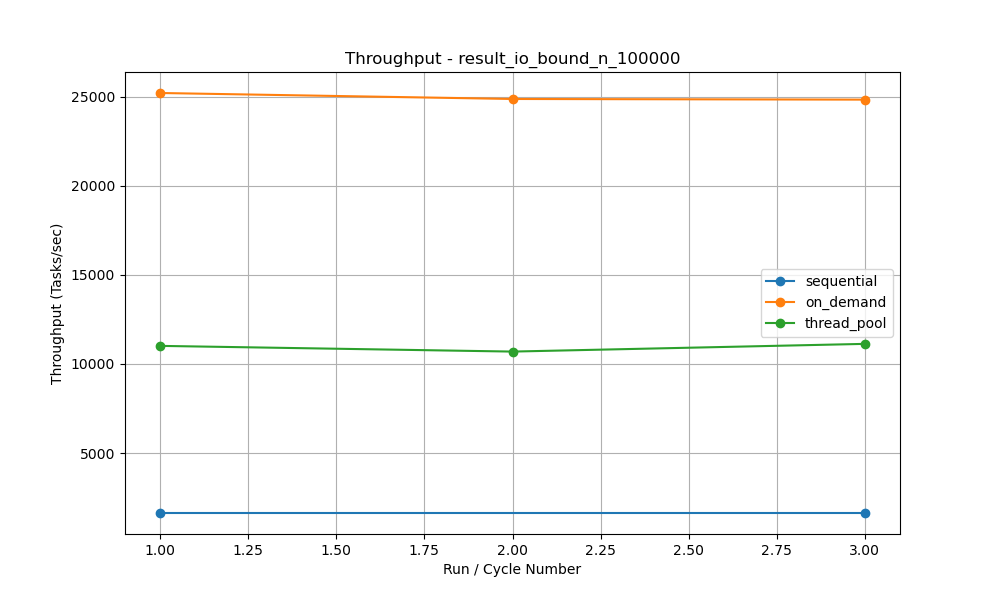
\includegraphics[width=0.82\linewidth]{benchmark/plot/io/throughput_result_io_bound_n_100000.png}
\caption{IO-bound throughput for the priority thread pool.}
\label{fig:io_throughput}
\end{figure}

\begin{figure}[htbp]
\centering
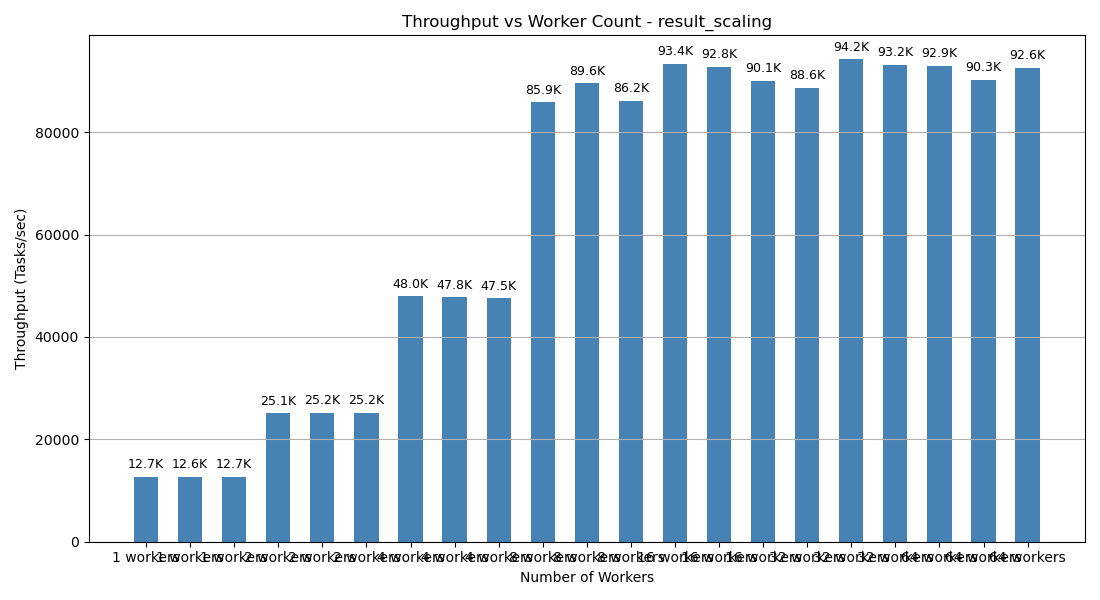
\includegraphics[width=0.82\linewidth]{benchmark/plot/scaling/throughput_result_scaling.png}
\caption{Worker scaling throughput for the priority thread pool.}
\label{fig:scaling_throughput}
\end{figure}

\begin{figure}[htbp]
\centering

\includegraphics[width=0.82\linewidth]{benchmark/plot/queue_ops/throughput_result_queue_ops.png}
\caption{Queue operation throughput for the priority thread pool.}
\label{fig:queue_ops_throughput}
\end{figure}

\begin{figure}[htbp]
\centering
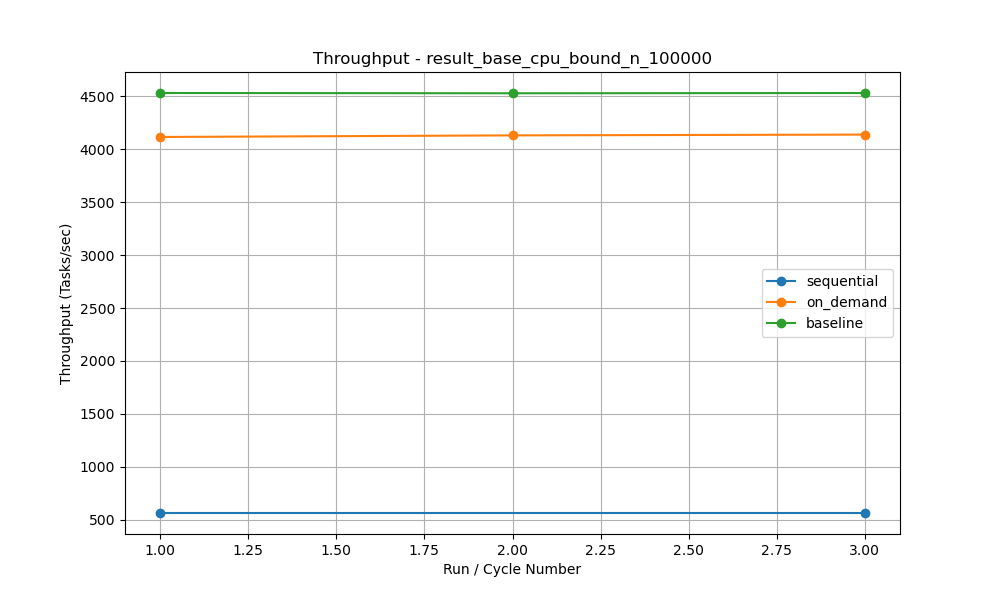
\includegraphics[width=0.82\linewidth]{benchmark/plot/baseline/cpu/throughput_result_base_cpu_bound_n_100000.png}
\caption{CPU-bound throughput for the FIFO baseline pool.}
\label{fig:baseline_cpu_throughput}
\end{figure}

\begin{figure}[htbp]
\centering
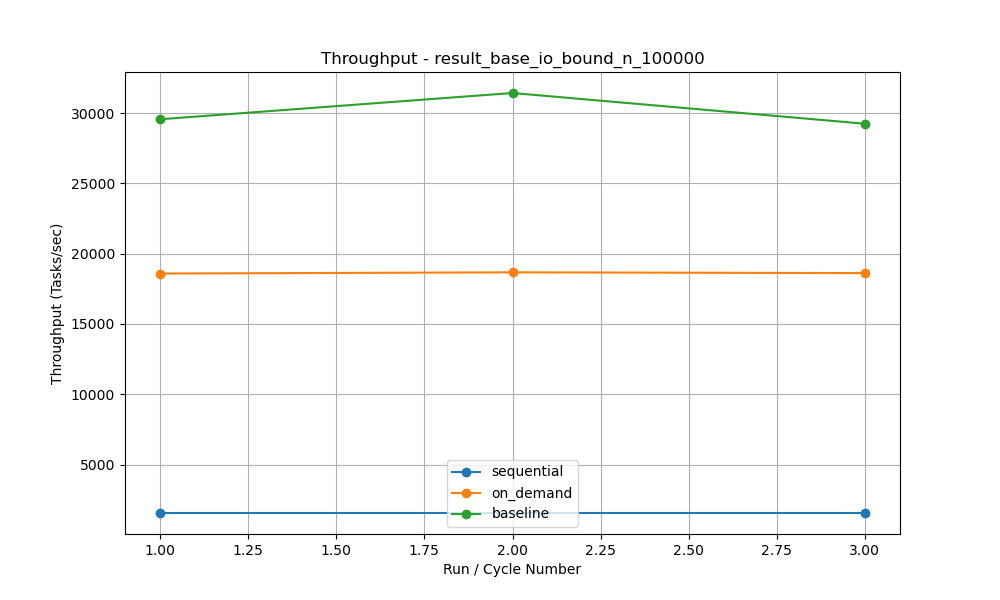
\includegraphics[width=0.82\linewidth]{benchmark/plot/baseline/io/throughput_result_base_io_bound_n_100000.png}
\caption{IO-bound throughput for the FIFO baseline pool.}
\label{fig:baseline_io_throughput}
\end{figure}

\begin{figure}[htbp]
\centering
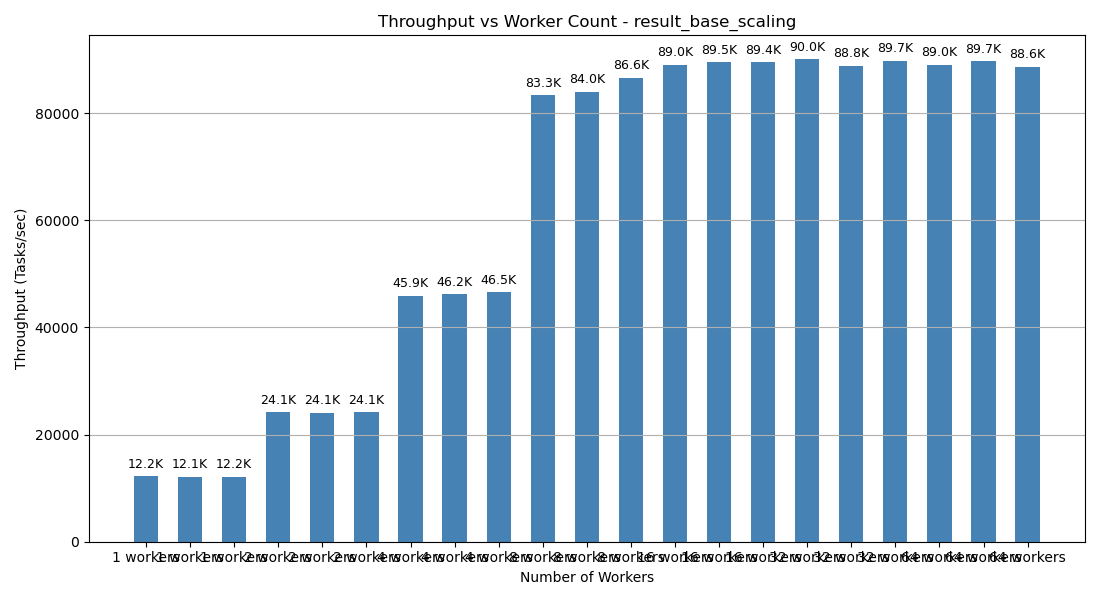
\includegraphics[width=0.82\linewidth]{benchmark/plot/baseline/scaling/throughput_result_base_scaling.png}
\caption{Worker scaling throughput for the FIFO baseline pool.}
\label{fig:baseline_scaling_throughput}
\end{figure}

\begin{figure}[htbp]
\centering

\includegraphics[width=0.82\linewidth]{benchmark/plot/baseline/queue_ops/throughput_result_base_queue_ops.png}
\caption{Queue operation throughput for the FIFO baseline pool.}
\label{fig:baseline_queue_ops_throughput}
\end{figure}

\begin{figure}[htbp]
\centering
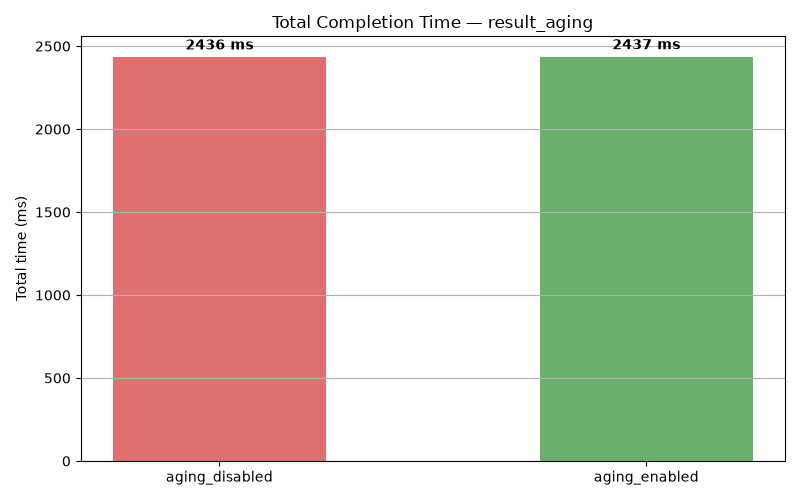
\includegraphics[width=0.82\linewidth]{benchmark/plot/aging/total_time_result_aging.png}
\caption{Total runtime with aging disabled and enabled.}
\label{fig:aging_total_time}
\end{figure}

\begin{figure}[htbp]
\centering
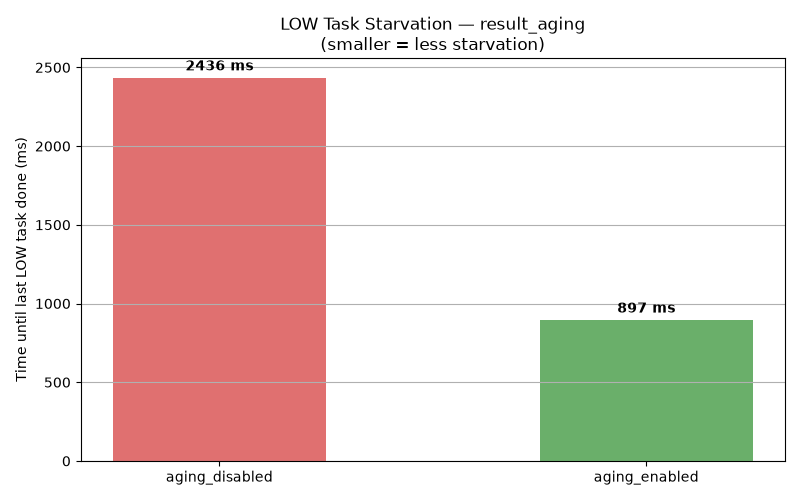
\includegraphics[width=0.82\linewidth]{benchmark/plot/aging/starvation_result_aging.png}
\caption{Low-priority starvation window with aging disabled and enabled.}
\label{fig:aging_starvation}
\end{figure}

\begin{figure}[htbp]
\centering
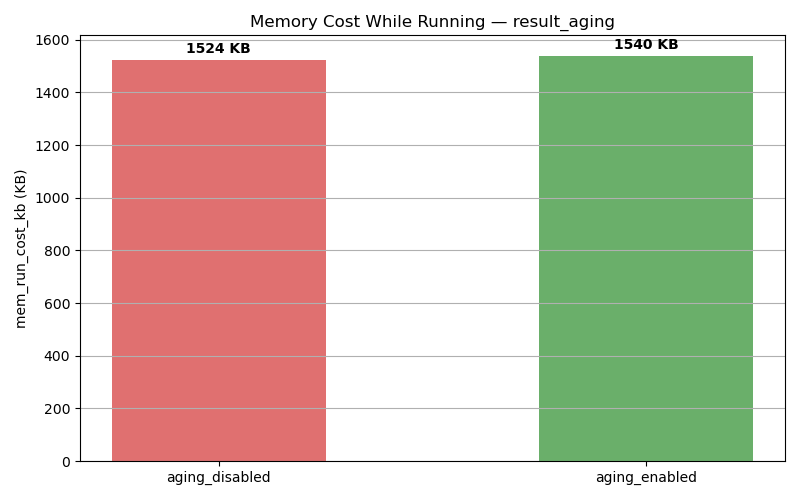
\includegraphics[width=0.82\linewidth]{benchmark/plot/aging/memory_result_aging.png}
\caption{Memory cost of the aging benchmark.}
\label{fig:aging_memory}
\end{figure}

\subsection{Analysis}

The fresh data shows that the priority pool is competitive on real workloads.
For CPU-bound Fibonacci work, it reaches 0.993x of the FIFO baseline, effectively
a tie. For the IO-bound workload, it reaches 1.014x, again within a narrow
competitive band. These results do not support a large real-workload throughput
gap between the two pools.

The strongest general-purpose advantage appears in worker scaling. Across 16,
32, and 64 workers, the priority pool reaches 1.031x, 1.028x, and 1.032x of
baseline throughput. This is lower than the expected 1.05x shape, but it is a
consistent advantage in the fresh dataset.

The inherent feature cost appears clearly in the queue-operation microbenchmark.
At one worker, the priority pool reaches only 0.699x of baseline queue throughput.
The gap narrows as contention rises, reaching 0.962x at 16 workers, but it does
not fully disappear in this run. This is the expected trade-off for richer
scheduling semantics: priority lanes, pause/resume support, monitoring, and
aging capability add overhead to a pure FIFO enqueue/dequeue path.

Predictability is mixed. The generated CPU and IO rows report 0.00\% CV for both
pools because the table generator used one selected pool-vs-baseline value for
those rows. Therefore this report does not claim the expected IO-bound CV
advantage. Queue-operation variance does show a clear stability advantage at
some worker counts: queue 4w is 2.21x more stable and queue 8w is 4.24x more
stable by the generated CV table.

The aging benchmark supports the fairness goal. Without aging, the last
low-priority task completes at 2493.2 ms on average. With aging enabled, it
completes at 922.5 ms on average, reducing the starvation window by about 2.70x.
Total runtime remains similar: 2493.2 ms without aging versus 2516.1 ms with
aging. This shows the scheduler improving fairness without materially changing
overall completion time in this workload.

Perf output is used only for explanation. The CPU-bound profile is dominated by
\texttt{fibonaccy}, matching the workload design. Queue-operation profiles show
kernel futex and scheduler-related overhead, consistent with synchronization
contention. IO profiles show page-cache and read-path activity. Syscall summary
views were attempted, but the machine denied raw syscall tracing permissions, so
they are not used for ranking.
